\chapter{Calibration}
\label{ch:calibration}

\section{\pmt}
\label{sec:pmt}

\todo{Pulseheight/integral, Number of particles. Leptons and gammas,
      separate?}

\subsection{LED calibration}
\label{sub:led_calibration}

We created a setup where an optical fiber is connected to a cap which
directs the light at the window of a \pmt to send bursts of photons at
it. This is similar to a pulse generator, but with light. The pulses are
created by LEDs and produce short (\SI{20}{\nano\second}) pulses with an
intensity comparable to one or two \mips in a detector, making them
similar to real scintillator signals. The pulse intensity or efficiency
fluctuates \todo[inline]{upto 50\%? due to LED or PMT?}. However,
averaged over 100 samples the pulse is very consistent
\todo[inline]{size of fluctuations on averages signal?}. A single fiber,
does not provide much control over the mean intensity and duration of
the pulses.

The setup provides 24 optical fibers, each with its own LED and slightly
different intensity. We have different caps that can be placed on a
\pmt. One cap allows for a single fiber to be connected while another
contains a bundle of many fibers allowing all 24 fibers to be used
simultaneously. Using the bundle of fibers each fiber looses about
\SI{25}{\percent} signal strength due to the fiber-to-fiber connection.
Signals of over \SI{5}{\volt} are possible with the bundle of fibers.

Since April 2014 each \pmt that is going to be used for a \hisparc
detector is first tested in the LED setup to ensure it responds properly
to light and that there is no significant background noise. The test
tries to find the voltage at which the pulses have a pulse height around
\SI{340}{\milli\volt}. This pulse height value requires a voltage close
to the normal operational voltage of \pmts on a \hisparc detector.


\subsection{Linearity}

In an EAS many more than one particle may pass through a detector. The
response of the \pmt to higher signals needs to be investigated to
determine the accuracy with which multiple particles can be
reconstructed. To increase the intensity multiple fibers can be combined
using the bundle of fibers. The setup is shown in \todo{add nice
photo/schematic of setup}. Each fiber is tested separately to determine
its mean intensity, then different combinations of multiple fibers are
combined as input. The expectation is that the individual intensities of
the fibers are simply added together. However, a \pmt might become
saturated or less efficient for larger signals, being unable to supply
the current quickly enough.

There are several types of \pmt being used in the \hisparc experiment.
Most established stations used \pmts that were fully created by outside
manufacturers. However, several batches have been encountered where the
power supply of the \pmt failed, while the tubes were still working
fine. The costs to replace the power supply were excessive. The \nikhef
Electronics department, which also developed the \hisparc electronics,
have worked on \pmt power supplies for the \kmnet neutrino telescope
experiment. The \kmnet \pmts have other requirements than those used for
\hisparc so some modifications were required. The \kmnet design has been
modified to be suitable for \hisparc. There have been a couple of
iteration of the \hisparc \pmts. Multiple \pmts of each of these
versions have been tested.

The tests show that the new \nikhef produced \pmt power supply can
supply enough current to saturate the \hisparc electronics. Moreover
they have a lineair response curve. The output corresponds to the sum of
the inputs. The old \pmts are lineair up to \SI{1}{\volt} (depending on
voltage). At higher signals they start showing diminishing returns,
barely reaching \SI{2.2}{\volt}. This effect can also be seen for some
\hisparc stations because the pulse height histogram does not reach the
maximum \adc value.

\begin{figure}
    \centering
    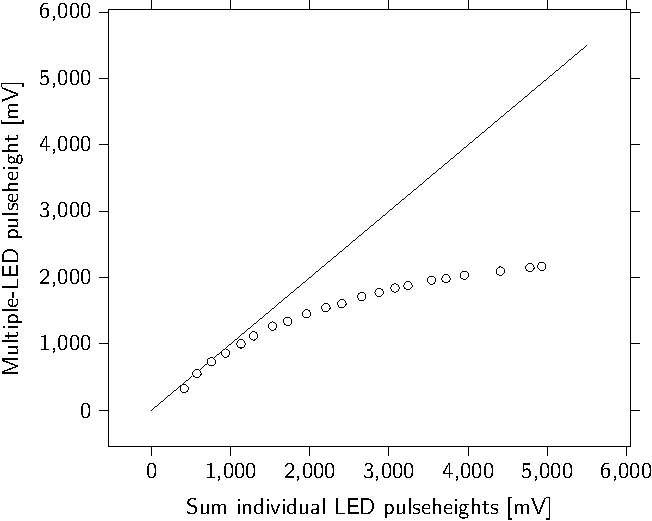
\includegraphics{plots/calibration/linearity_senstech_ph}
    \caption{Measurements of the pulse height linearity.}
    \label{fig:linearity_senstech_ph}
\end{figure}

From the detector data can already see non-linearity by plotting the
measured pulse heights against the pulse integrals for the same events
\todo[inline]{figure showing the ph v pi}. For the old \pmts this
already showed that the pulse height is not lineair. However, it does
not show if the pulse integral is lineair or not. By measuring the pulse
heights and integrals using the setup we can see show non-lineair they
both are.

\begin{figure}
    \centering
    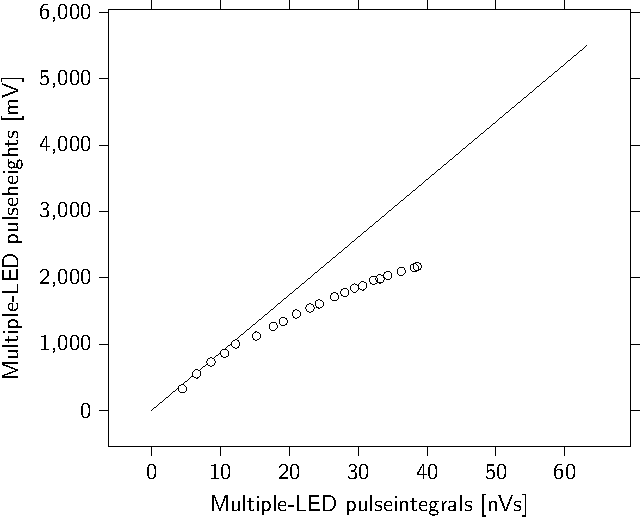
\includegraphics{plots/calibration/linearity_senstech_ph_pi}
    \caption{Measurements of the pulse height versus pulse integral.}
    \label{fig:linearity_senstech_ph_pi}
\end{figure}

The \adcs in the \hisparc electronics are designed and calibrated to
make the range \SIrange{200}{4096}{\Adc} correspond to the range
\SIrange{0}{-2}{\volt}. Signals greater than \SI{-2}{\volt} are clipped,
preventing the pulse height to provide an accurate measure of signal
strength. The clipping also affects the pulse integral, however, bigger
signals are often also wider, contributing to the pulse integral.

\todo{Using ND-filters to weaken the signal, to check for walk
      (arrival time determination).}


\section{\gps accuracy}
\label{sec:gps_accuracy}

Time difference calibration measurements have been performed on
HiSPARC II and III electronic boxes. This started after dr. David
Fokkema discovered an unexpected time offset between timestamps of
events in a test where two HiSPARC stations (501 and 502) were triggered
with the same pulse generator (Fokkema 2012 p47). Since these stations
are very close ($\sim\SI{100}{\meter}$) a minimal time offset was
expected, any offset or large standard deviation was expected to be the
result of errors in \gps accuracy and position. However, a large offset
($\Delta t \sim\SI{18}{\nano\second}$) was found. Further tests have
been performed to determine the cause of the offset, these tests are
described in this section. Both the \hisparc electronics and \gps
antennas were found to have varying offsets contributing to time
differences in the resulting time measurements.


\subsection{Making timestamps}
\label{sub:gps_timestamps}

%\citep{Verkooijen:2008tq}
In the report Message Structures \hisparc the method used for
determining the time for an event is thoroughly explained. Every second
the \gps receiver sends a signal (a Pulse Per Second) to the \hisparc
electronics. The \hisparc box uses a $\SI{200}{\mega\hertz}$ clock to
determine the time within this second. Since the crystal in this clock
does not work at exactly $\SI{200}{\mega\hertz}$ the counter (reset at
the arrival of a PPS) is read at the moment of an event and then when
the next PPS arrives. Giving information about at what fraction of that
second the event occured. For higher accuracy (more than
$\SI{5}{\nano\second}$) the clock is also read on the negative side of
the clock, making the system clock an effective
$\SI{400}{\mega\hertz}$ clock.

\begin{equation}
    Timestamp = E_{Sync} + E_{Quan1} + \left(\frac{T_{Event}}{T_{PPS}}\right)
                 \left(1e^9 - E_{Quan1} + E_{Quan2}\right)
\end{equation}

Where $E_{Quan}$ is the Quantization Error, $E_{Sync}$ is the
Synchronization Error, $T_{Event}$ are the count of ticks till the event
and $T_{PPS}$ are the count of ticks between the PPS before and after
the event.

\todo{Explain 3 one second messages are needed to make timestamp. Messages Structures HiSPARC p.2}


\subsection{Test setup}
\label{sub:gps_test_setup}

In the setup one \hisparc II Master (hardware serial: 62) is used as the
main reference point for the entire test. All other \hisparc boxes were
tested against this reference one at a time to measure the offset. Two
\gps antennas ('501' and 'test') and a \gps splitter were used. With
these it was possible to perform tests in which both \hisparc boxes used
the same \gps antenna, removing the offset caused by using different
\gps antennas.

Each \hisparc box was connected to a \gps antenna and a PC, each running
the current version of the \hisparc Software; \hisparc DAQ II v3.0.4.
When the \hisparc III boxes needed to be tested the DAQ was upgraded to
the beta version of the new DAQ; \hisparc DAQ III v1.0.0.

A \SI{100}{\mega\hertz} Pulse Generator (as reference: Tabor Electronics
Model 8600), with two short equal-length signal cables and a signal
splitter was used to trigger the \hisparc electronics. Each box was
connected to the same pulse generator through either of the PMT input
channels. To ensure the generated signals arrived at the same time at
the input both cables from the pulse generator were connected to the
same \hisparc electronics and also switched around.

\begin{figure}
    \centering
     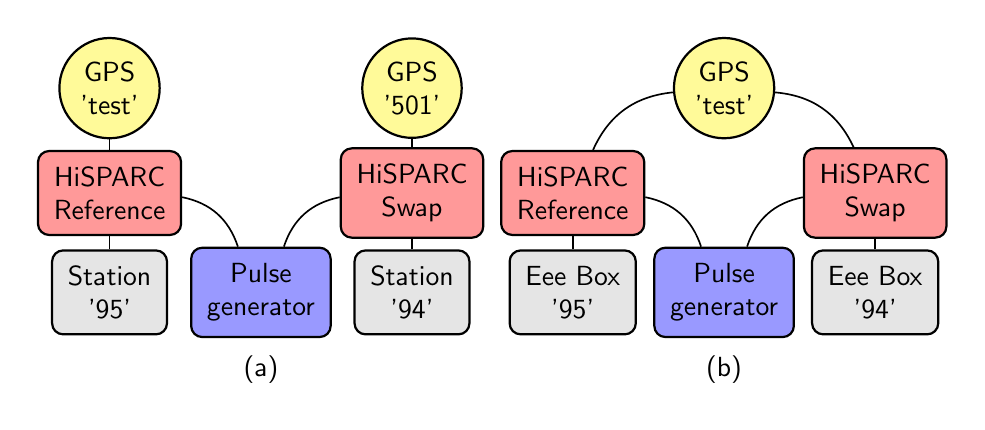
\begin{tikzpicture}
  [font=\sffamily,
   every matrix/.style={ampersand replacement=\&,column sep=0.1cm,row sep=0.1cm},
   gps/.style={draw,thick,circle,fill=yellow!40,inner sep=.1cm, align=center},
   pc/.style={draw,thick,rounded corners,fill=black!10,inner sep=.2cm, align=center},
   hisparc/.style={draw,thick,rounded corners,fill=red!40,inner sep=.2cm, align=center},
   pulse/.style={draw,thick,rounded corners,fill=blue!40,inner sep=.2cm, align=center},
   to/.style={-,semithick,font=\sffamily\footnotesize},]

  \matrix{
   \node[gps] (test) {GPS\\'test'}; \& \& \node[gps] (501) {GPS\\'501'}; \& \& \& \node[gps] (b_test) {GPS\\'test'}; \& \\
   \node[hisparc] (refr) {HiSPARC\\Reference}; \& \& \node[hisparc] (swap) {HiSPARC\\Swap}; \& \& \node[hisparc] (b_refr) {HiSPARC\\Reference}; \& \& \node[hisparc] (b_swap) {HiSPARC\\Swap}; \\
   \node[pc] (95) {Station\\'95'}; \& \node[pulse] (pulse) {Pulse\\generator}; \& \node[pc] (94) {Station\\'94'}; \& \& \node[pc] (b_95) {Eee Box\\'95'};  \& \node[pulse] (b_pulse) {Pulse\\generator}; \& \node[pc] (b_94) {Eee Box\\'94'}; \\
   \& \node {(a)}; \& \& \& \& \node {(b)}; \& \\
  };
  
  \draw[to] (test) -- node[below,above,sloped] {} (refr);
  \draw[to] (501) -- node[below,above,sloped] {} (swap);
  \draw[to] (95) -- node[midway,midway,sloped] {} (refr);
  \draw[to] (94) -- node[midway,midway,sloped] {} (swap);
  \draw[to] (pulse) to[bend left] node[above,below,sloped] {} (swap);
  \draw[to] (pulse) to[bend right] node[above,below,sloped] {} (refr);

  \draw[to] (b_test) to[bend right] node[below,above,sloped] {} (b_refr);
  \draw[to] (b_test) to[bend left] node[below,above,sloped] {} (b_swap);
  \draw[to] (b_95) -- node[midway,midway,sloped] {} (b_refr);
  \draw[to] (b_94) -- node[midway,midway,sloped] {} (b_swap);
  \draw[to] (b_pulse) to[bend left] node[above,below,sloped] {} (b_swap);
  \draw[to] (b_pulse) to[bend right] node[above,below,sloped] {} (b_refr);

 \end{tikzpicture}

    \caption{This image shows the setup of the test, two HiSPARC PCs
             with HiSPARC Masters (Reference and Swap), both connected
             to the same pulse generator. Each is also connected to a
             \gps, some tests used separate \gps antennas (a) and in
             some tests the same \gps was used by both (b).}
    \label{fig:setup}
\end{figure}


\subsection{Offsets between \hisparc electronics}
\label{sub:gps_offsets}

Tests to determine the offset distribution between \hisparc electronics
have been performed using a \gps splitter to ensure they see the same
\gps signal.

Found slightly varying offsets between each \hisparc electronics unit.
Constant over time. Can be corrected with enough statistics.
Importance of 24 hour self-survey. - Do many 1 hour tests

\todo{Test again year later, same difference??}

The offsets in the \hisparc electronics can be as high as $|\Delta t| =
\SI{15}{\nano\second}$. While the $\sigma_{\Delta t}$ remains within GPS
specifications ($\sigma_{\Delta t} < \SI{4.5}{\nano\second}$).

\todo{Time offset caused by \gps, 501-510 example, \gps swapped}

\gps cable twists affect signal speed?

\begin{figure}
    \centering
    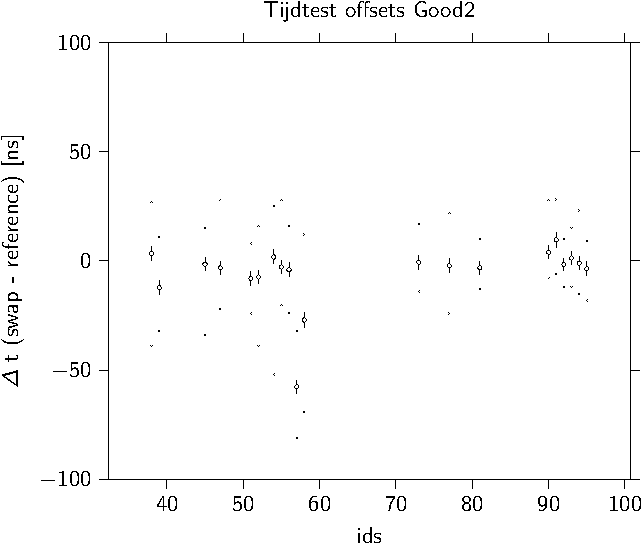
\includegraphics{plots/calibration/hisparc_offsets}
    \caption{Time offsets relative to a reference box. Circles are the
             mean offsets, the error bars the standard deviation and the
             points indicate the minimum and maximum of the test.}
    \label{fig:hisparc_offsets}
\end{figure}


\subsection{Corrections}

The offset can be determined from real data. For any combination of two
stations the expected mean time difference of all coincident events is,
because of mirror symmetry, \SI{0}{\nano\second}. However the spread
around the mean is very dependent on the distance between the stations,
because showers at an angle will create larger time differences if the
stations are further apart. Moreover, the increased distance means that
less events will be detected simultaneously by both stations because
showers of higher energy and larger footprints occur less often. To
determine the offset between stations that are further apart more data
is required.
